The CEED uses Bakeoff Problems (BPs) to test and compare the performance of high-order finite element implementations.
The definitions of these bakeoff problems are given on the CEED website \cite{ceed-bps} and are summarized in Table \ref{table:ceedbps}.

\begin{table}[ht!]
\begin{center}
\begin{tabular}{l l c c}
  \toprule
  BP  & Problem         & components & quadrature points  \\
  \toprule
  BP1 & mass matix      & $1$        & $q = p + 2$        \\
  BP2 & mass matix      & $3$        & $q = p + 2$        \\
  \midrule
  BP3 & stiffness matix & $1$        & $q = p + 2$        \\
  BP4 & stiffness matix & $3$        & $q = p + 2$        \\
  \midrule
  BP5 & stiffness matix & $1$        & $q = p + 1$        \\
  BP6 & stiffness matix & $3$        & $q = p + 1$        \\
  \bottomrule
\end{tabular}
\end{center}
\caption{CEED Bakeoff Problems}
\label{table:ceedbps}
\end{table}

In these BPs, the stiffness matrix is given by the Laplacian.
These problems use nodal bases on the Gauss-Legendre-Lobatto points with order $p$ nodal basis functions with $q$ quadrature points in each dimension for a total of $\left( p + 1 \right)^d$ nodes and $q^d$ quadrature points, where $d$ is the dimension of the problem.
For BP5 and BP6 the quadrature points are collocated with the nodal points.
Since the collocated quadrature is appropriate for a smaller range of practical applications, we will focus on results for BP1, BP2, BP3, and BP4.

\begin{figure}[ht!]
\begin{subfigure}{.99\textwidth}
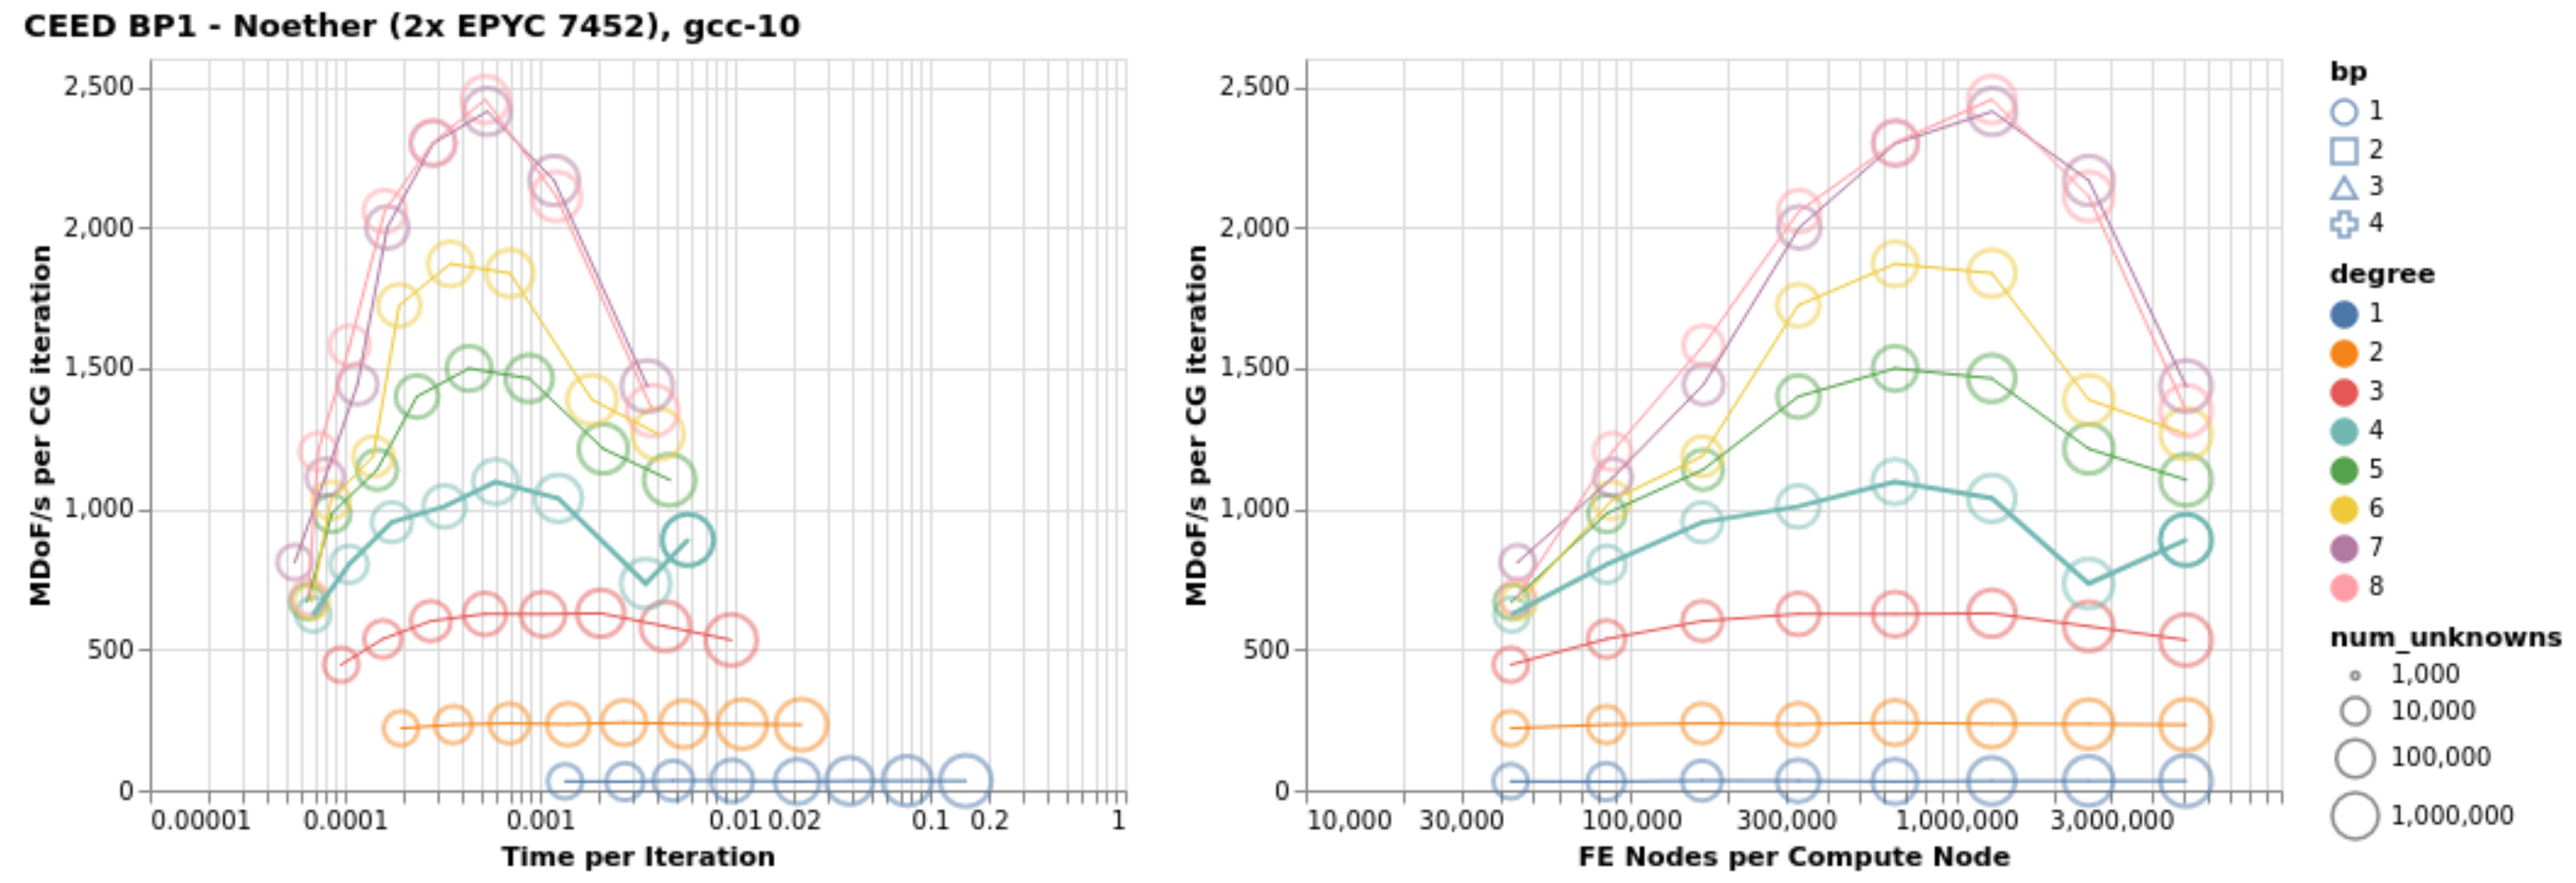
\includegraphics[width=.99\linewidth]{../img/xsmmSerialBP1Clip}
\caption{Serial XSMM Backend}
\end{subfigure}\\
\begin{subfigure}{.99\textwidth}
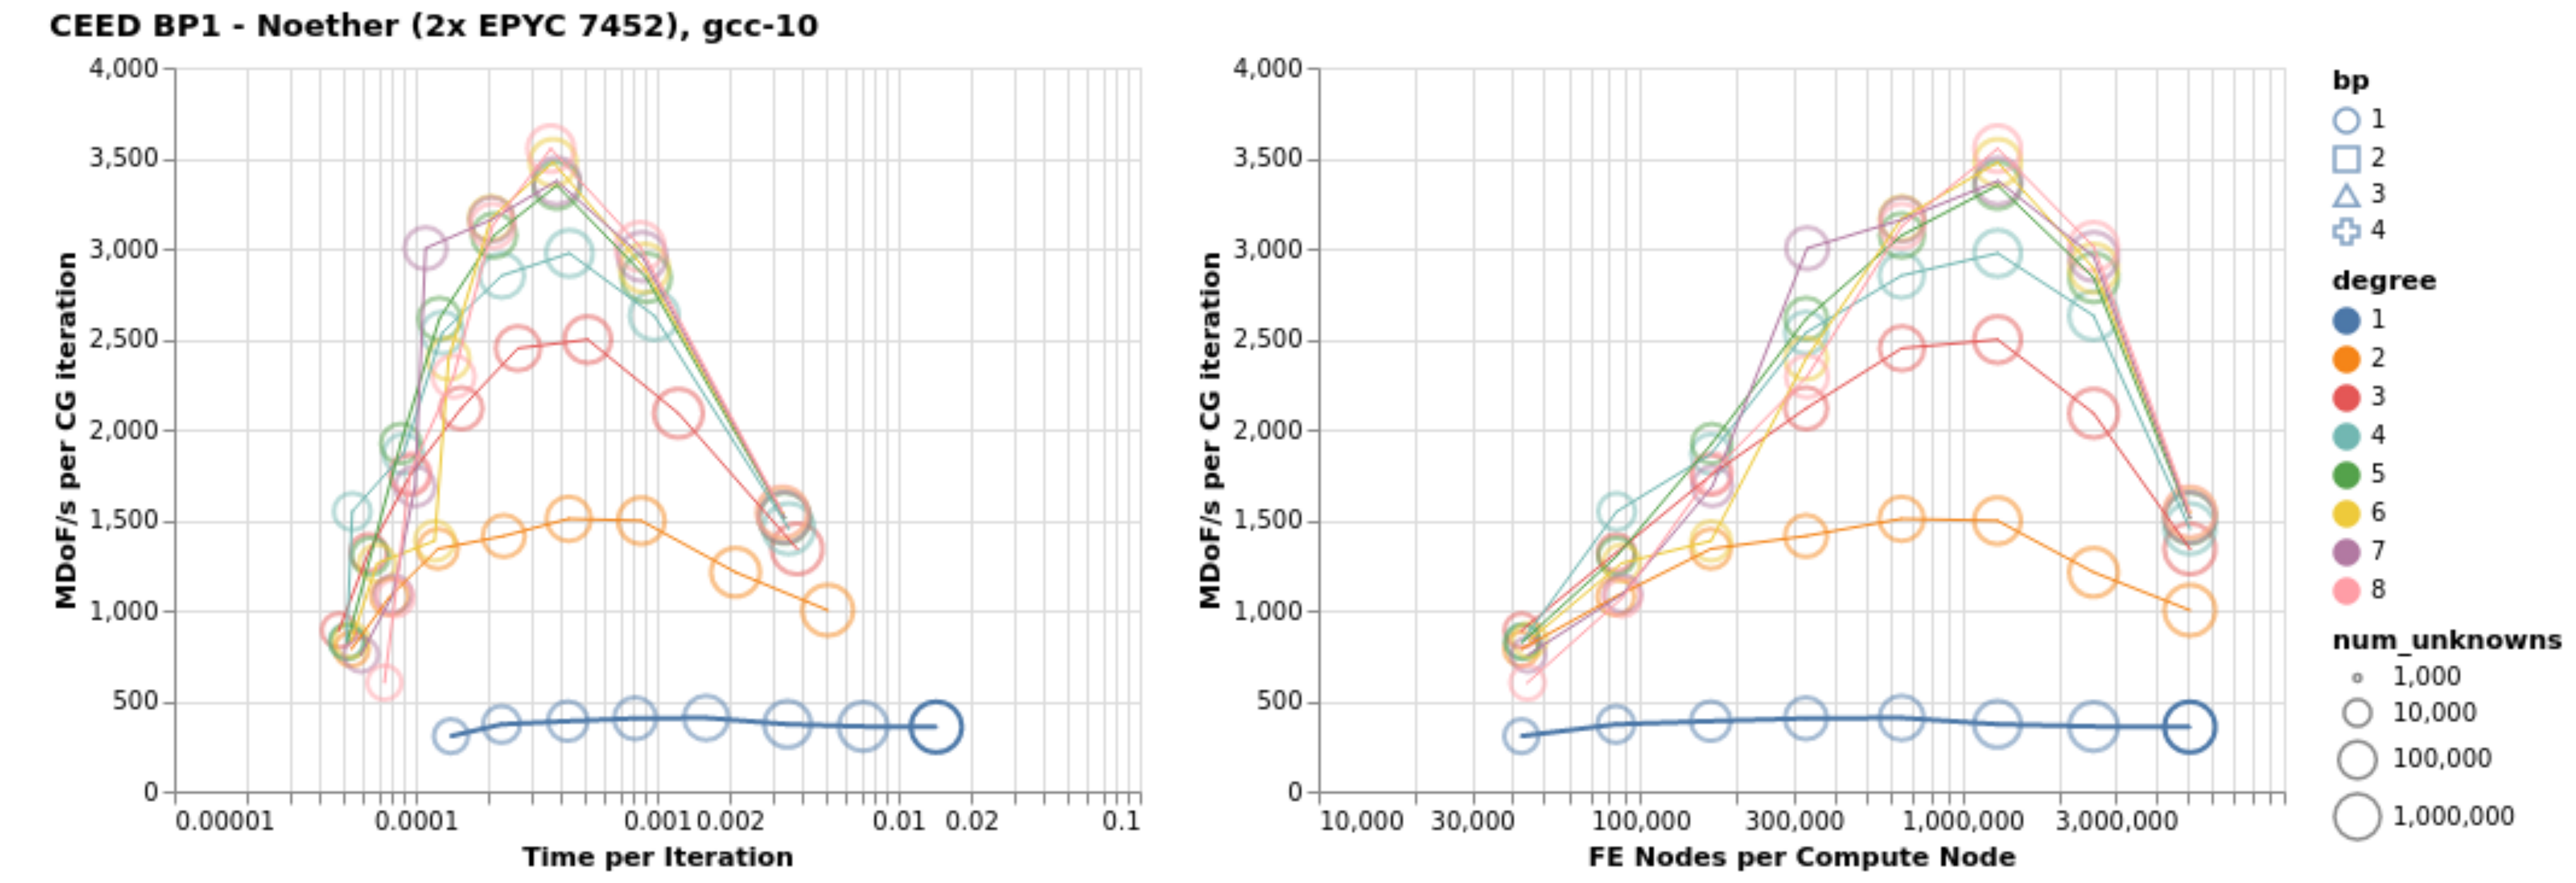
\includegraphics[width=.99\linewidth]{../img/xsmmBlockedBP1Clip}
\caption{Blocked XSMM Backend}
\end{subfigure}
\caption{CEED Benchmark BP1 - AMD EPYC}
\label{fig:cpu-bp1}
\end{figure}

\begin{figure}[ht!]
\begin{subfigure}{.99\textwidth}
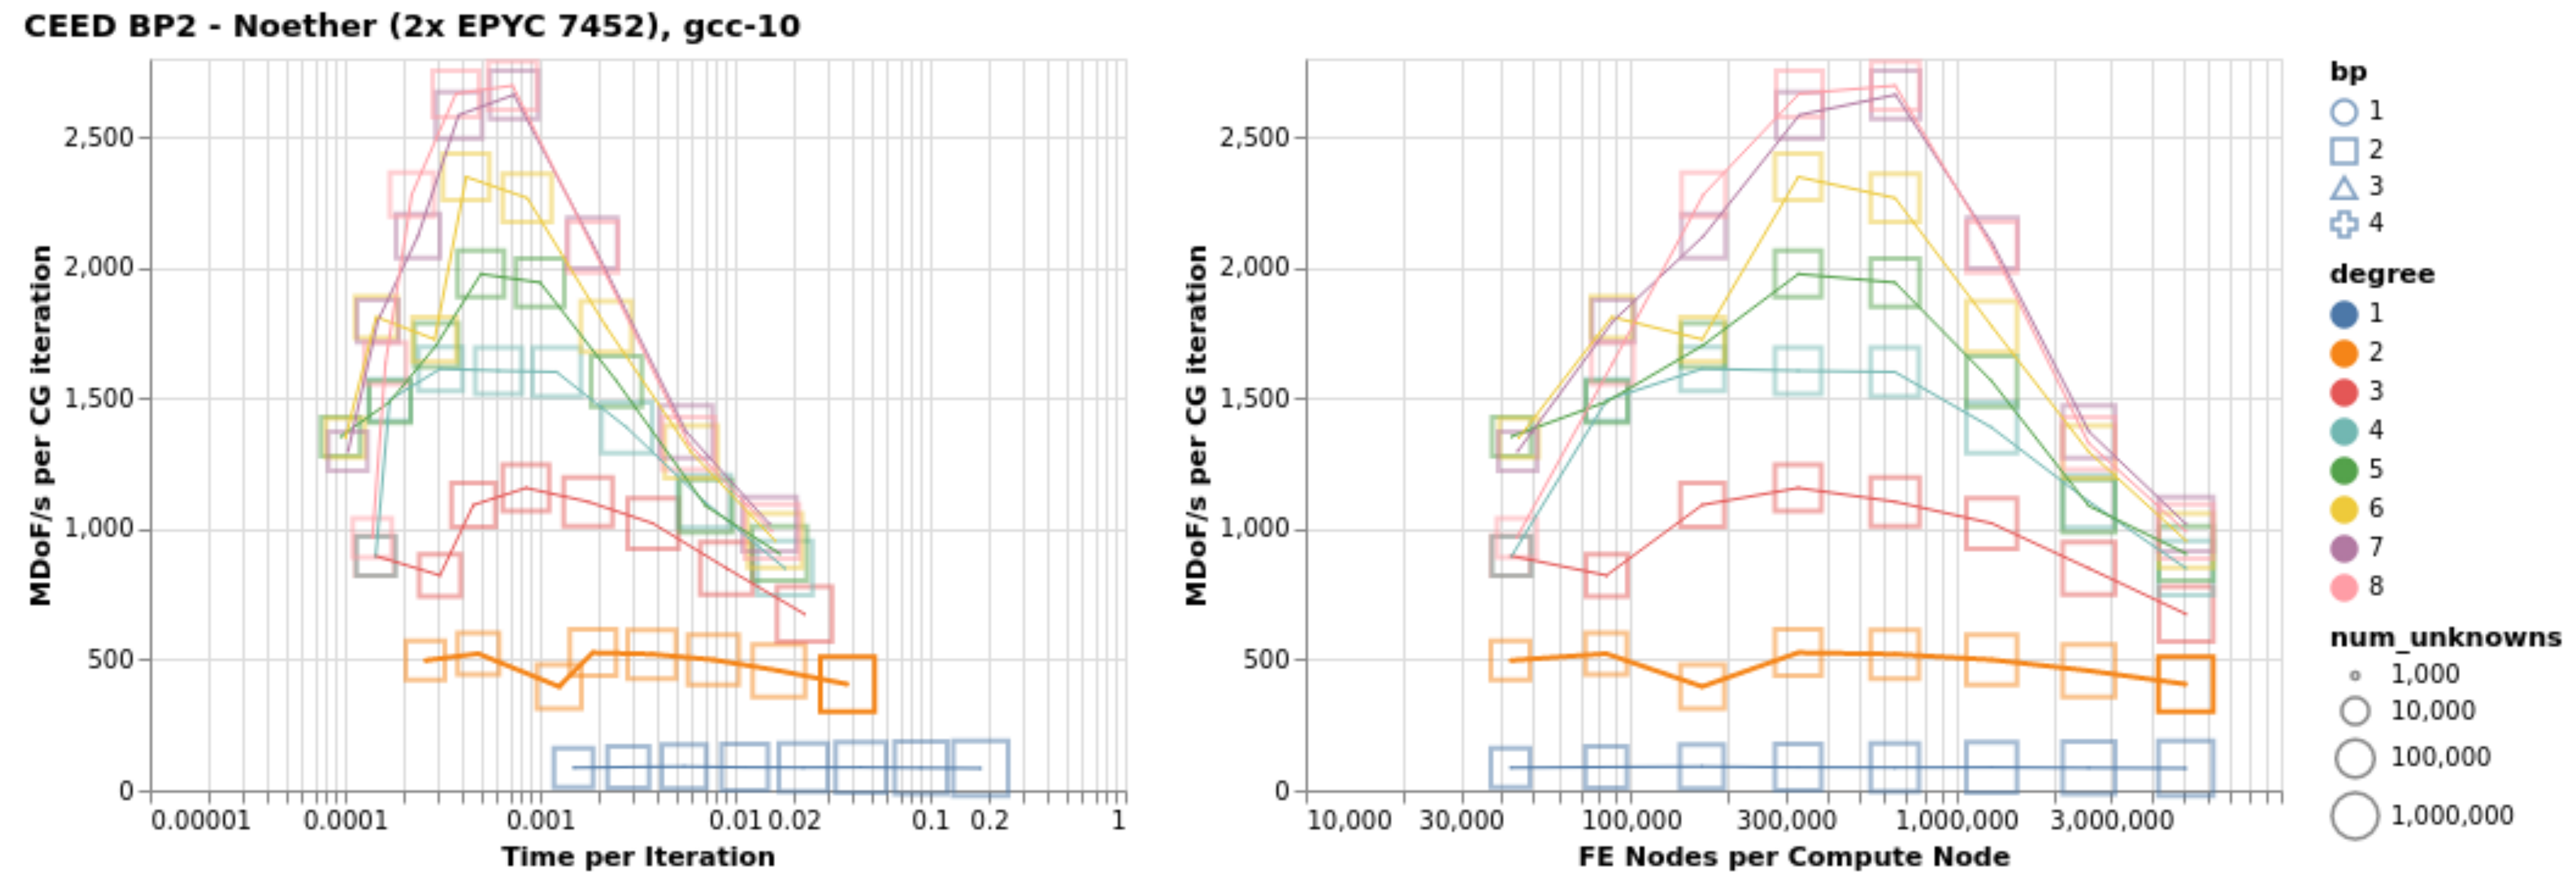
\includegraphics[width=.99\linewidth]{../img/xsmmSerialBP2Clip}
\caption{Serial XSMM Backend}
\end{subfigure}\\
\begin{subfigure}{.99\textwidth}
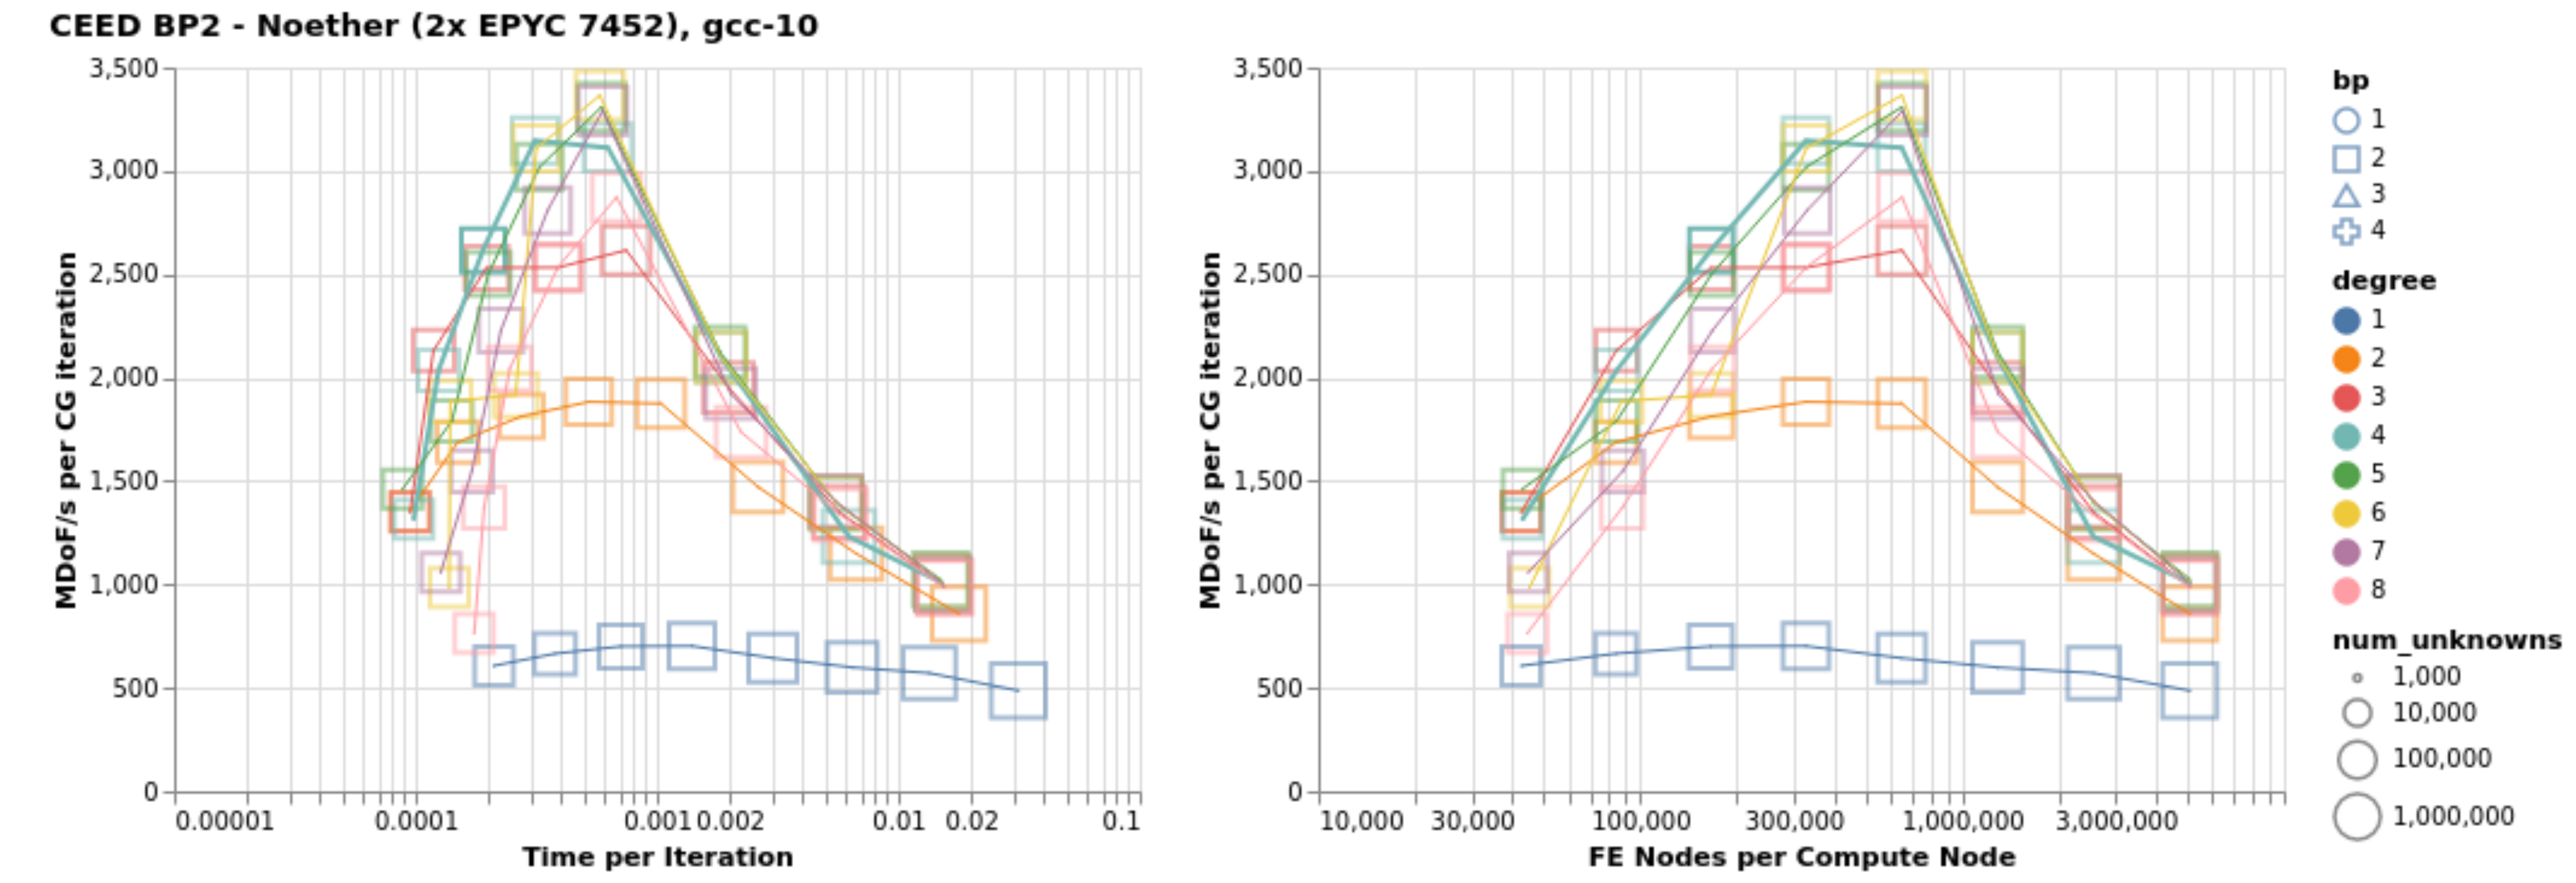
\includegraphics[width=.99\linewidth]{../img/xsmmBlockedBP2Clip}
\caption{Blocked XSMM Backend}
\end{subfigure}
\caption{CEED Benchmark BP2 - AMD EPYC}
\label{fig:cpu-bp2}
\end{figure}

\begin{figure}[ht!]
\begin{subfigure}{.99\textwidth}
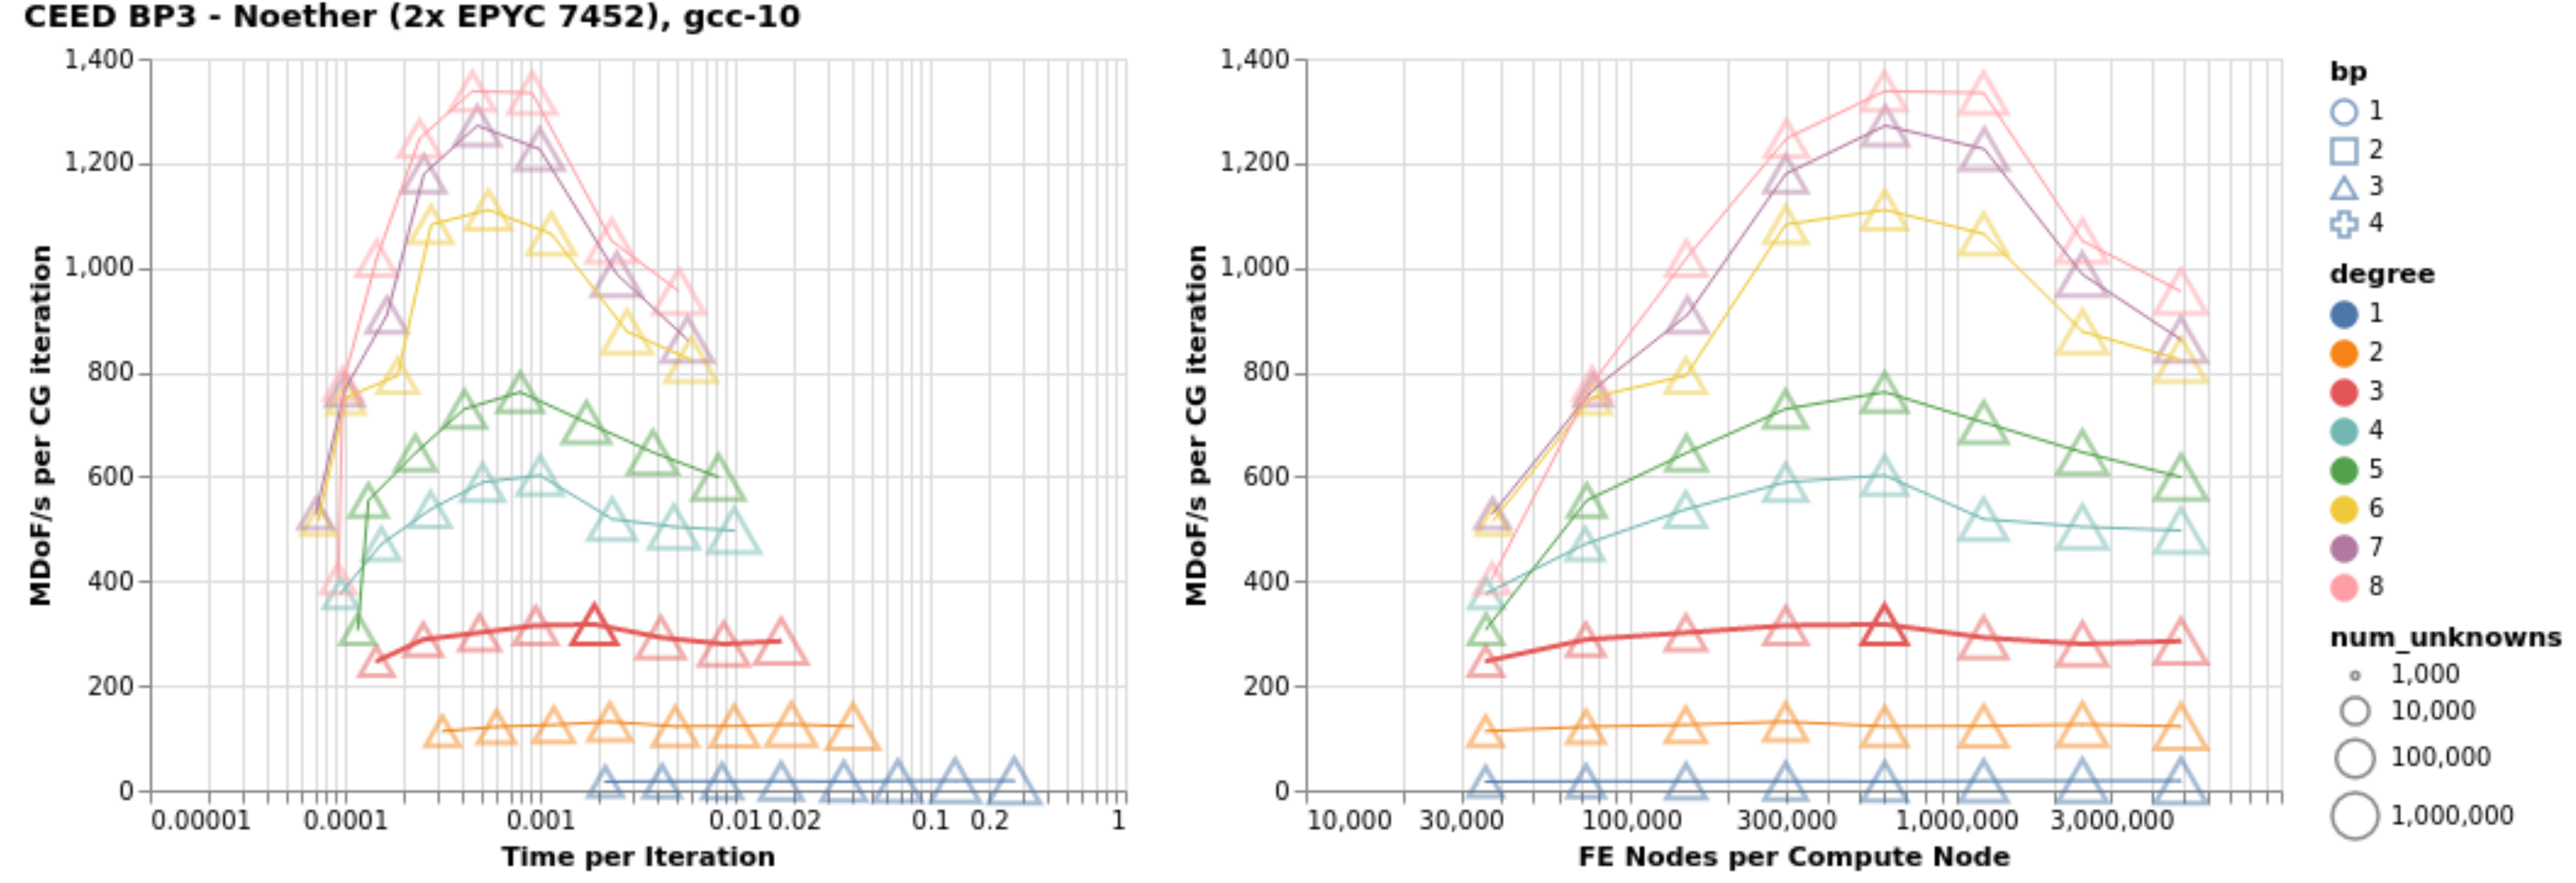
\includegraphics[width=.99\linewidth]{../img/xsmmSerialBP3Clip}
\caption{Serial XSMM Backend}
\end{subfigure}\\
\begin{subfigure}{.99\textwidth}
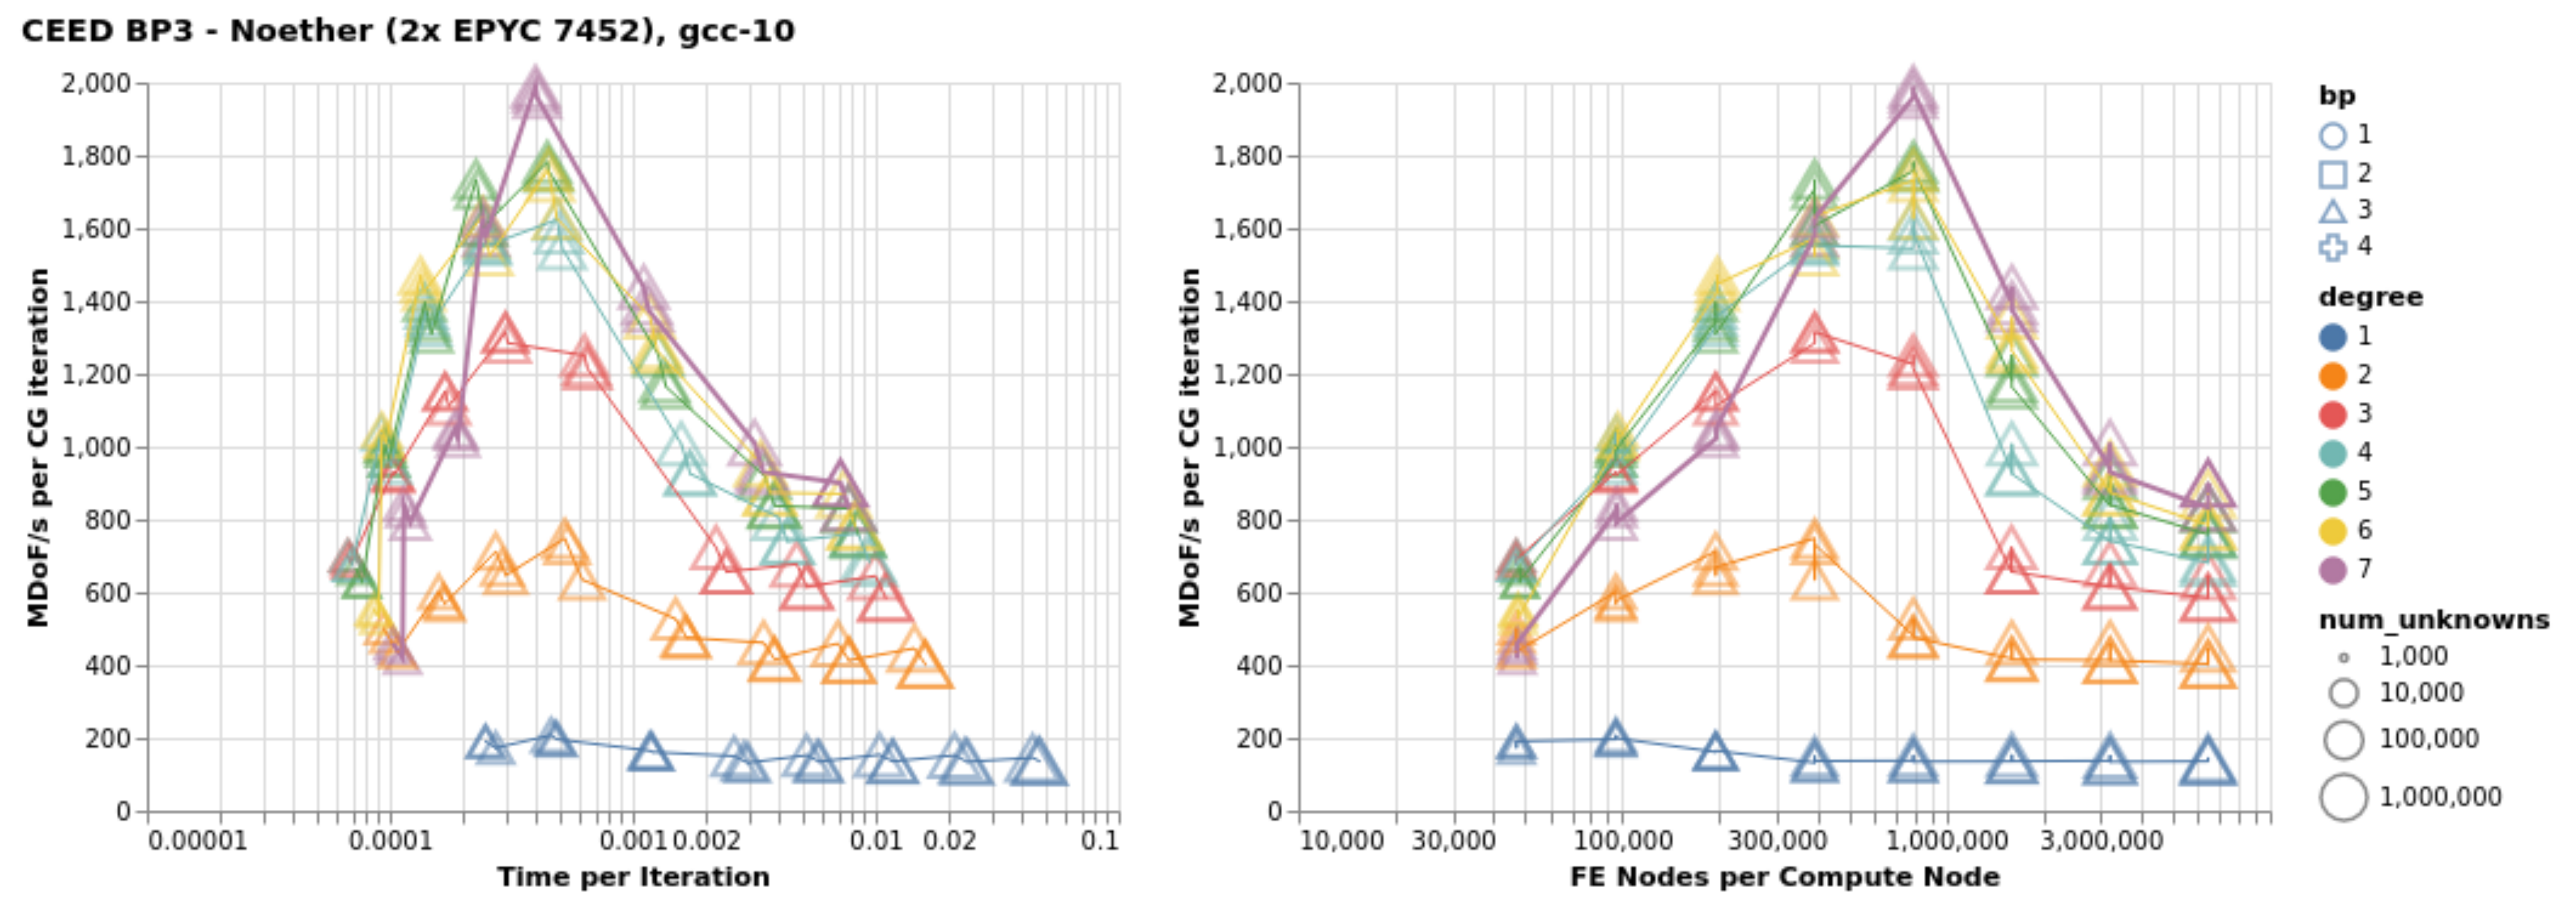
\includegraphics[width=.99\linewidth]{../img/xsmmBlockedBP3Clip}
\caption{Blocked XSMM Backend}
\end{subfigure}
\caption{CEED Benchmark BP3 - AMD EPYC}
\label{fig:cpu-bp3}
\end{figure}

\begin{figure}[ht!]
\begin{subfigure}{.95\textwidth}
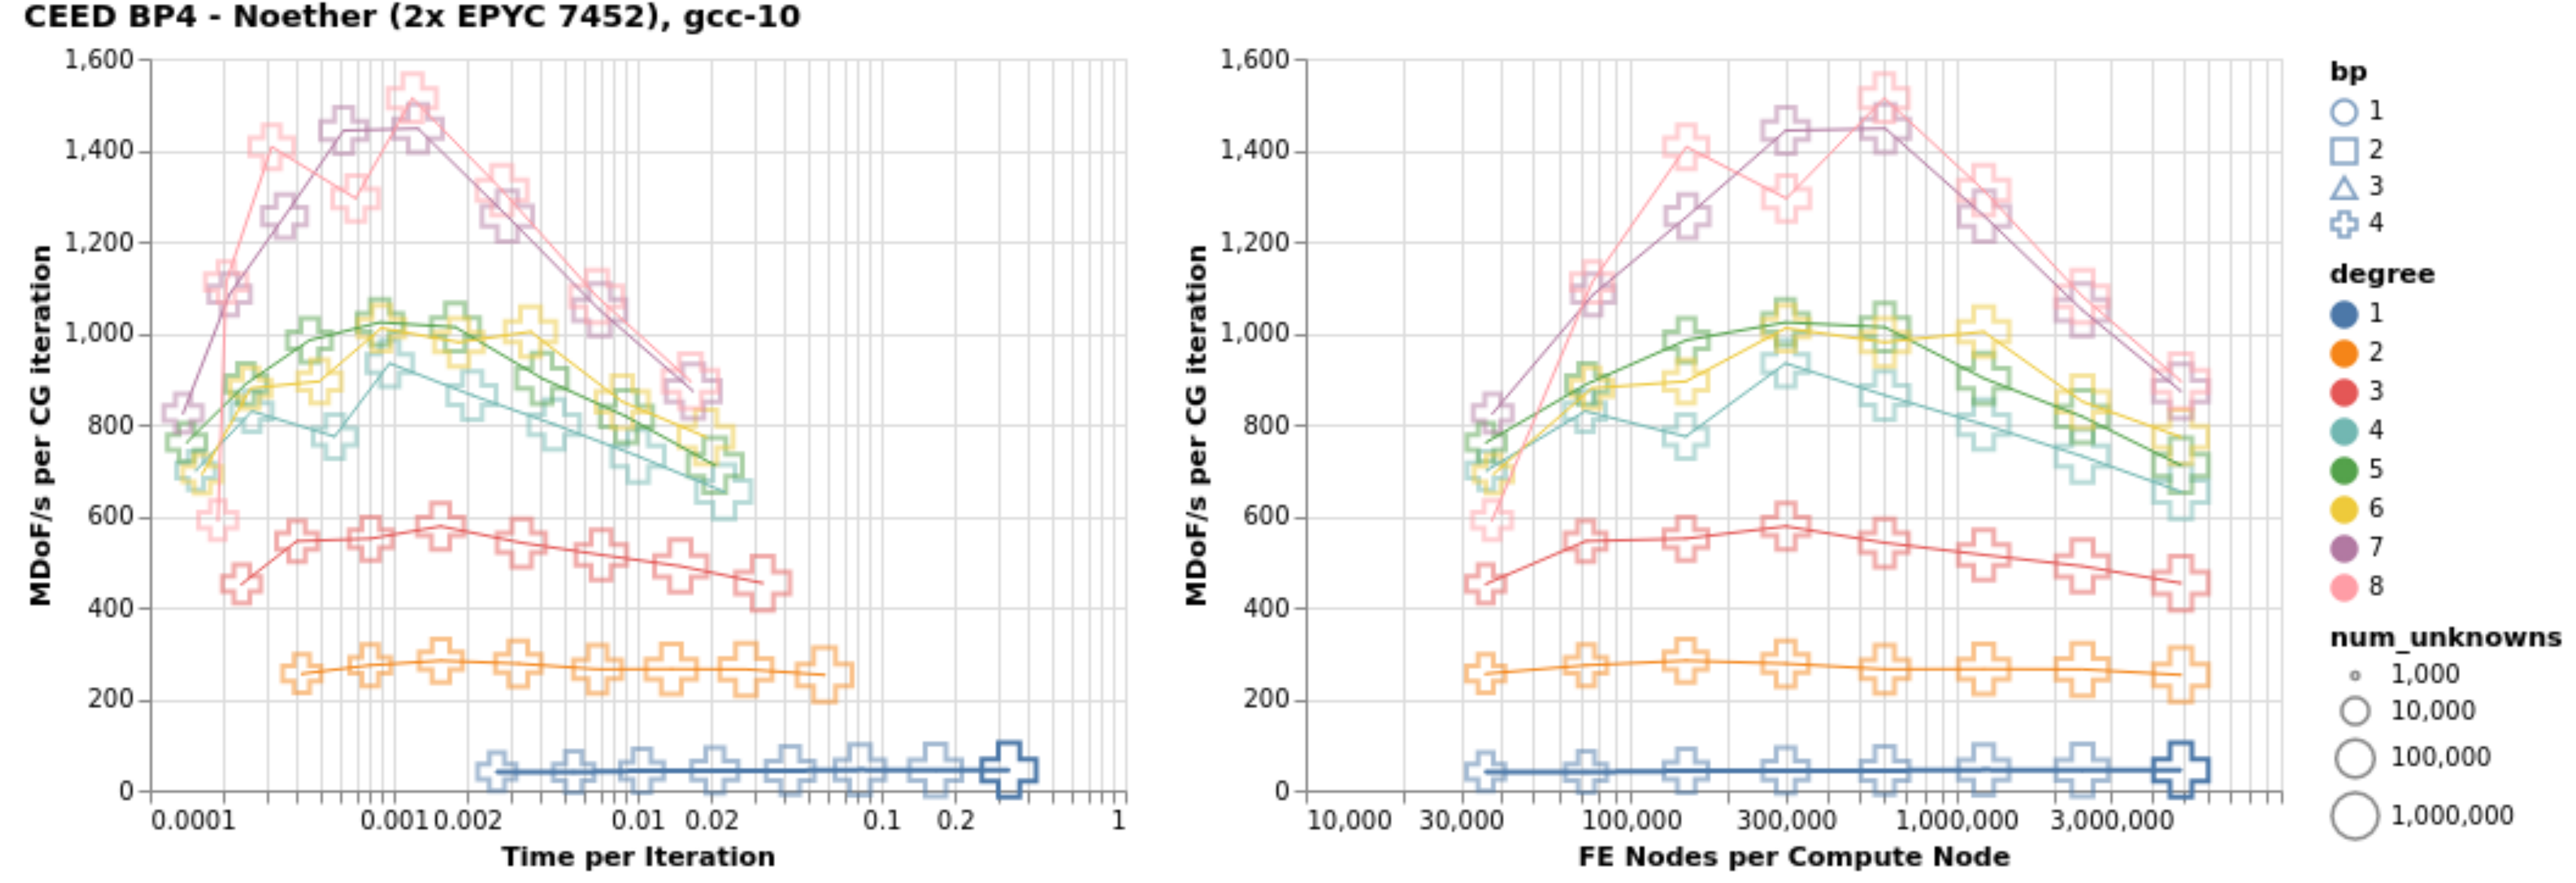
\includegraphics[width=.99\linewidth]{../img/xsmmSerialBP4Clip}
\caption{Serial XSMM Backend}
\end{subfigure}\\
\begin{subfigure}{.95\textwidth}
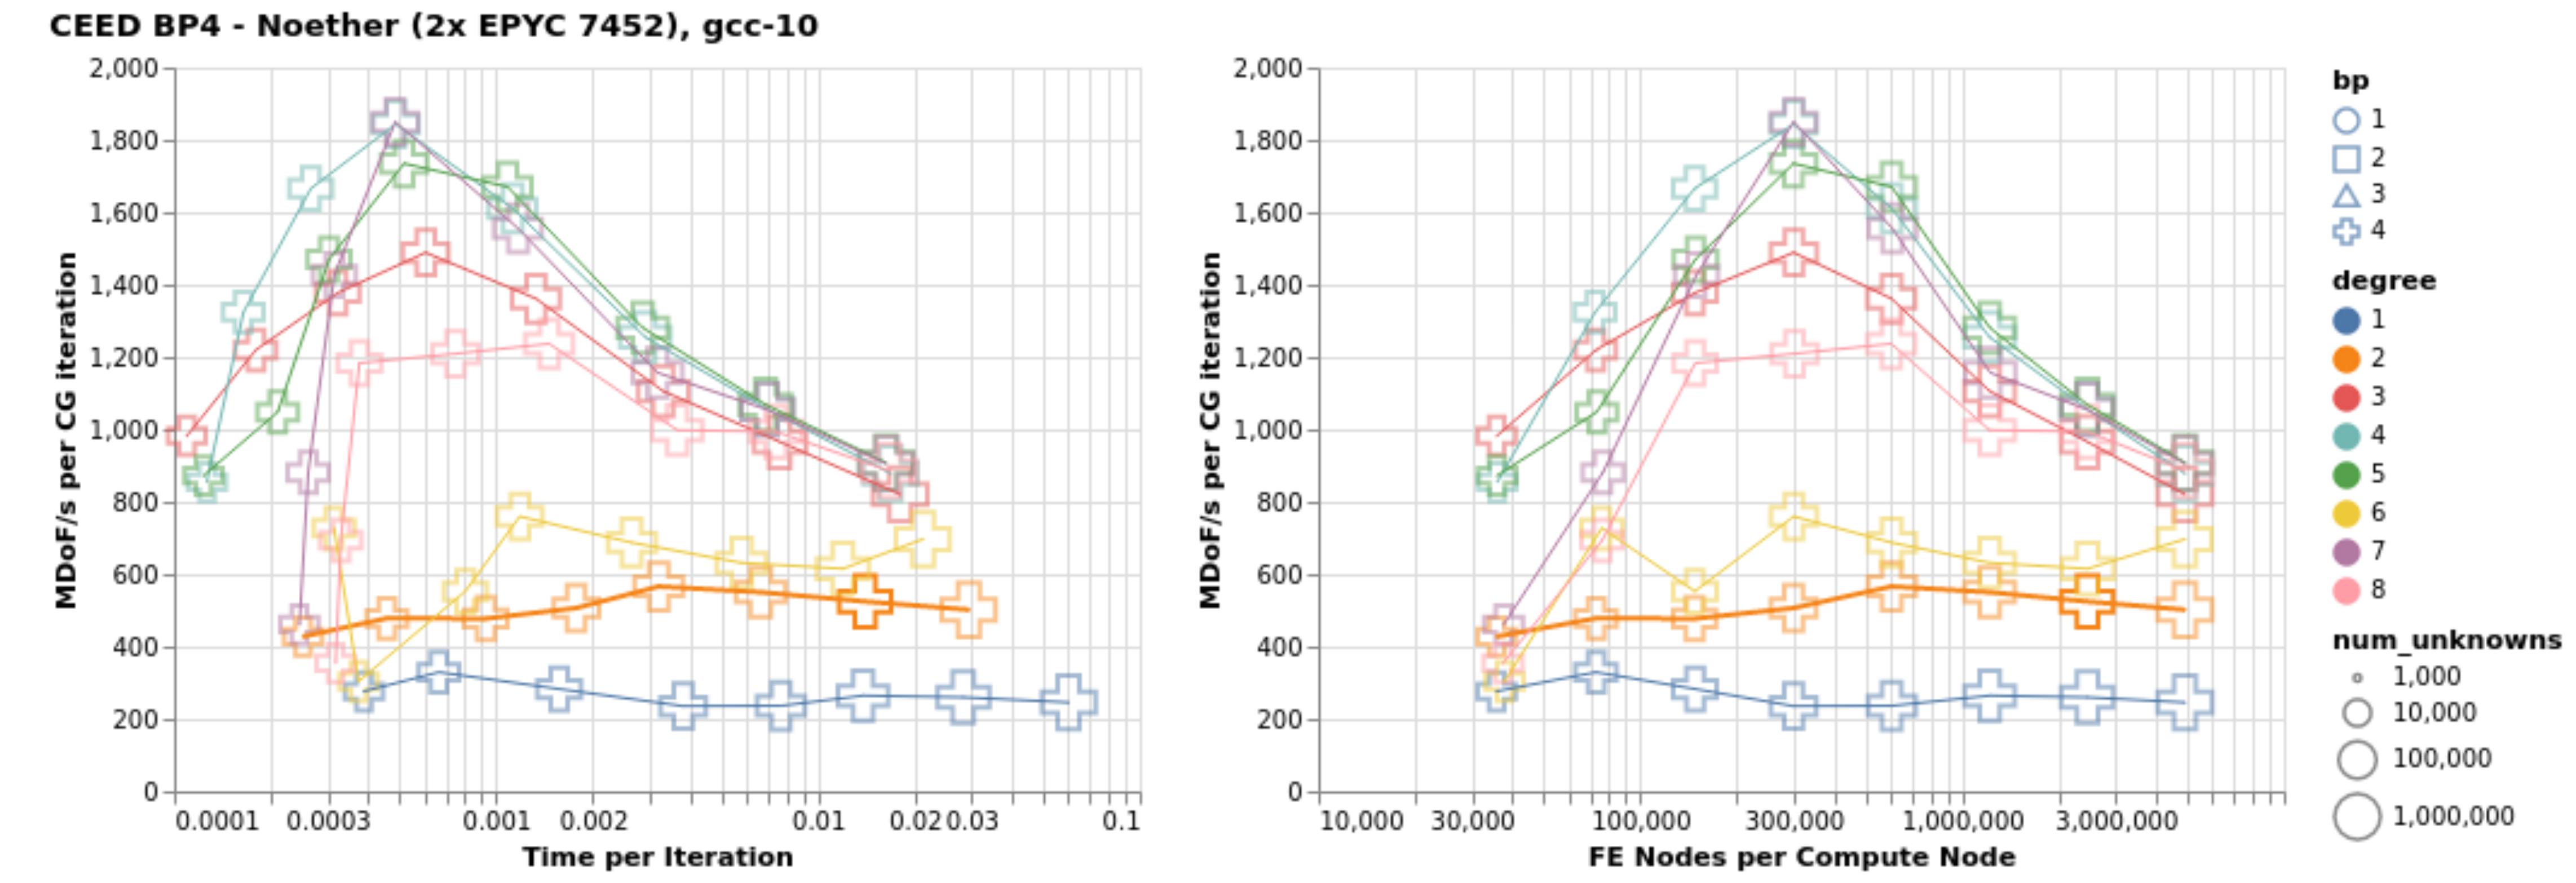
\includegraphics[width=.99\linewidth]{../img/xsmmBlockedBP4Clip}
\caption{Blocked XSMM Backend}
\end{subfigure}
\caption{CEED Benchmark BP4 - AMD EPYC}
\label{fig:cpu-bp4}
\end{figure}

The CPU performance study was conducted on a machine with two-socket AMD EPYC 7452 machine.
Figures \ref{fig:cpu-bp1}, \ref{fig:cpu-bp2}, \ref{fig:cpu-bp3}, and \ref{fig:cpu-bp4} show the results of this performance study.
Each socket contains 32 CPU cores with a base clock speed of 2.35 GHz and 128 MB of L3 cache.
The NPS4 BIOS configuration was used and processes were bound to cores.
MPICH-3.3.2 was used with PETSc \cite{petsc-user-ref} version 3.15 and libCEED \cite{libceed} version 0.9.

libCEED used the serial and blocked LIBXSMM \cite{libxsmm} backends, \lstinline{\cpu\self\xsmm\serial} and \lstinline{\cpu\self\xsmm\blocked}.
In the serial backends, elements are in sequence and operations are vectorized across the data for a single element while in the blocked backends elements are interlaced in 8 element batches to facilitate vectorization.
LIBXSMM Just in Time (JiT) compilation of small matrix-matrix product kernels using Advanced Vector Extensions (AVX) instructions to provide high-performance tensor product evaluations on CPU architecture.

Figure \ref{fig:cpu-bp1} shows the results for CEED BP1.
As anticipated, we see higher throughput as the polynomial order of the basis increases.
The high throughput with low latency indicates that this architecture demonstrates good strong scaling, while high throughput with high latency would indicate that the architecture weak scales effectively.

In Figure \ref{fig:cpu-bp2} we see the results for CEED BP2.
For this problem, throughput starts to drop off for the blocked backend as the polynomial order of the bases increases above $p = 6$.
This is because the 8 element batch on the 3 component vector problem is large enough to spill out of the cache on this architecture.
This is an indication that for this polynomial order the single element batching strategy used by the serial element processing LIBXSMM backend, \lstinline{\cpu\self\xsmm\serial}, would be more appropriate.

In Figure \ref{fig:cpu-bp3} and Figure \ref{fig:cpu-bp4}, we see a similar behavior, but for the more computationally intensive Laplacian rather than the mass matrix.
In this case, the throughput in the 3 component vector problem drops off after the polynomial order of the bases increases above $p = 5$.

\begin{figure}[ht!]
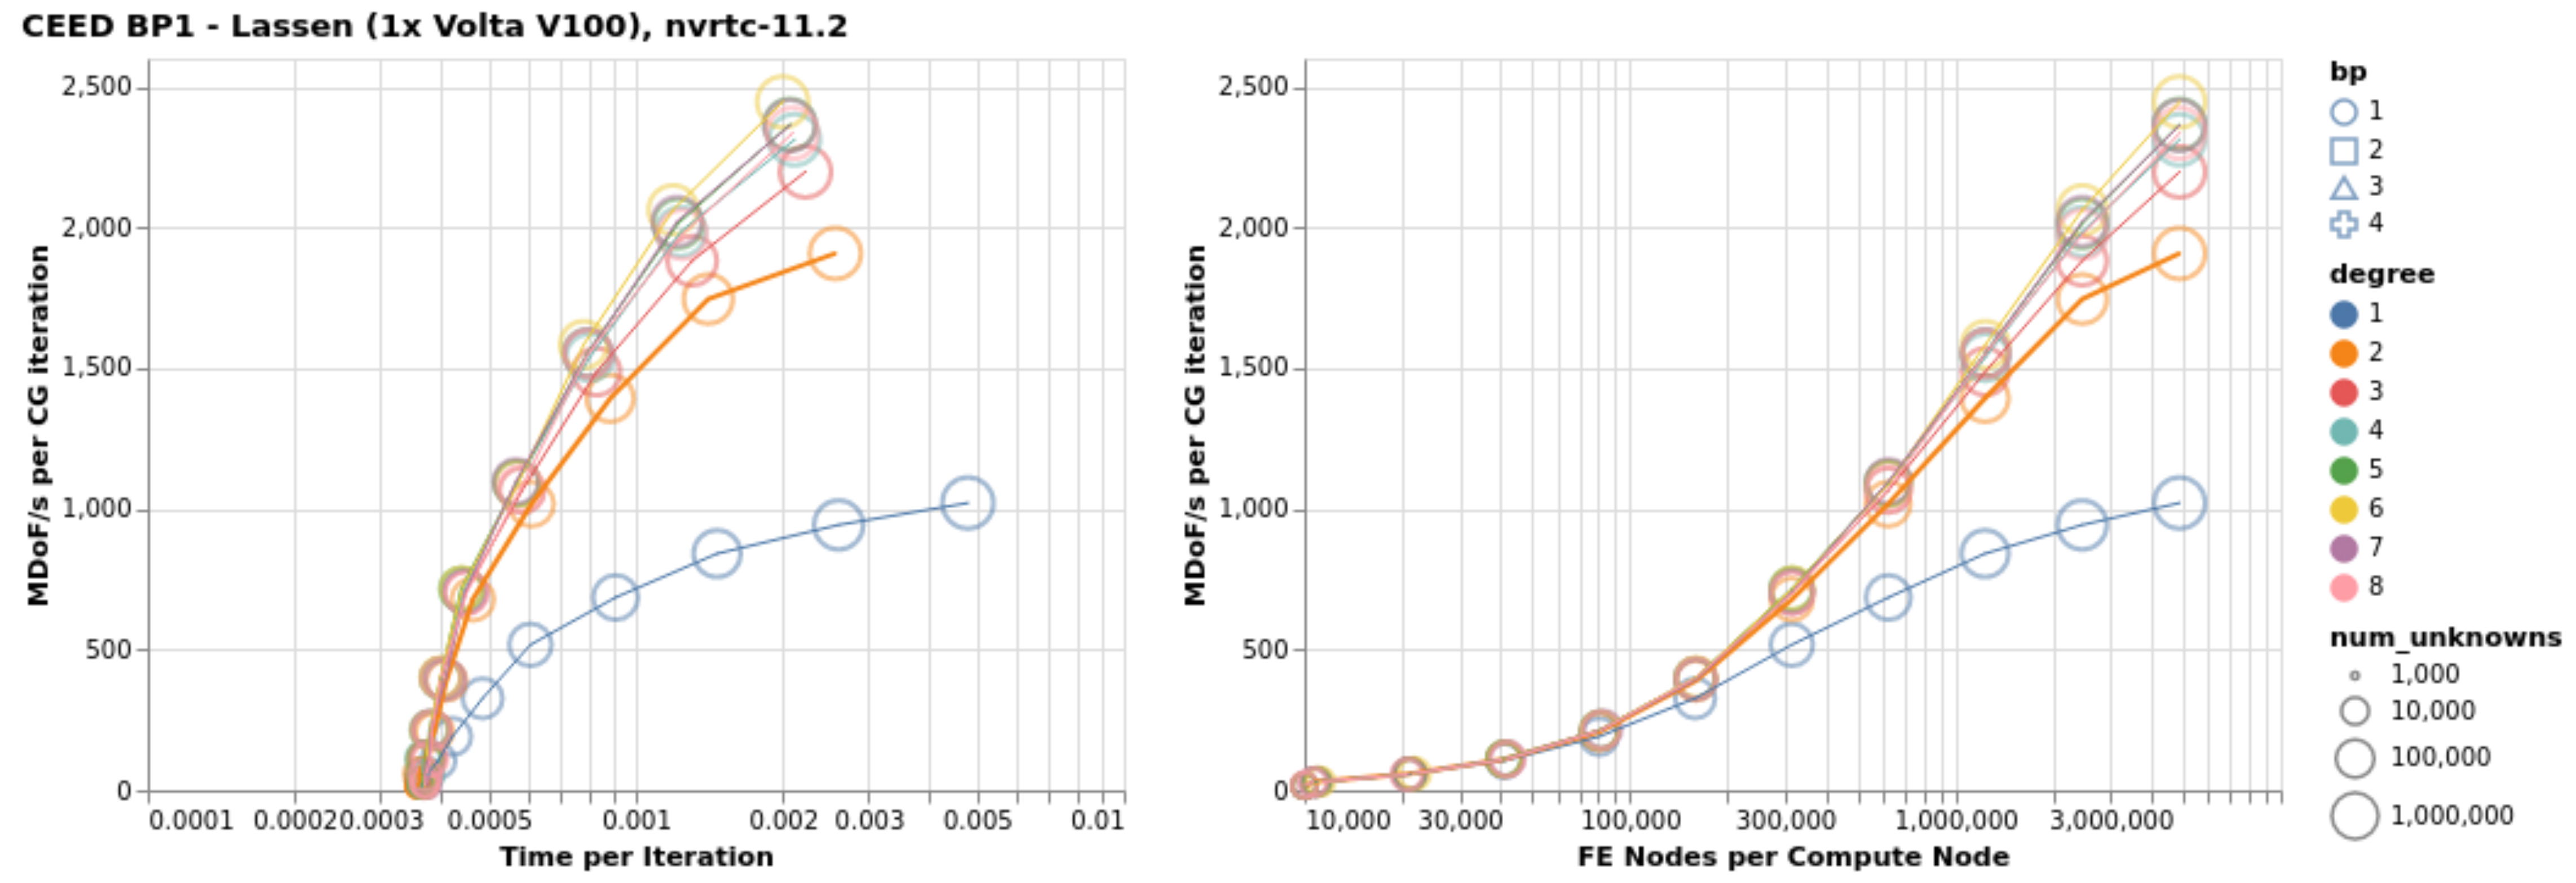
\includegraphics[width=.99\linewidth]{../img/cudaGenBP1Clip}
\caption{CEED Benchmark BP1 - NVIDIA V100}
\label{fig:gpu-bp1}
\end{figure}

\begin{figure}[ht!]
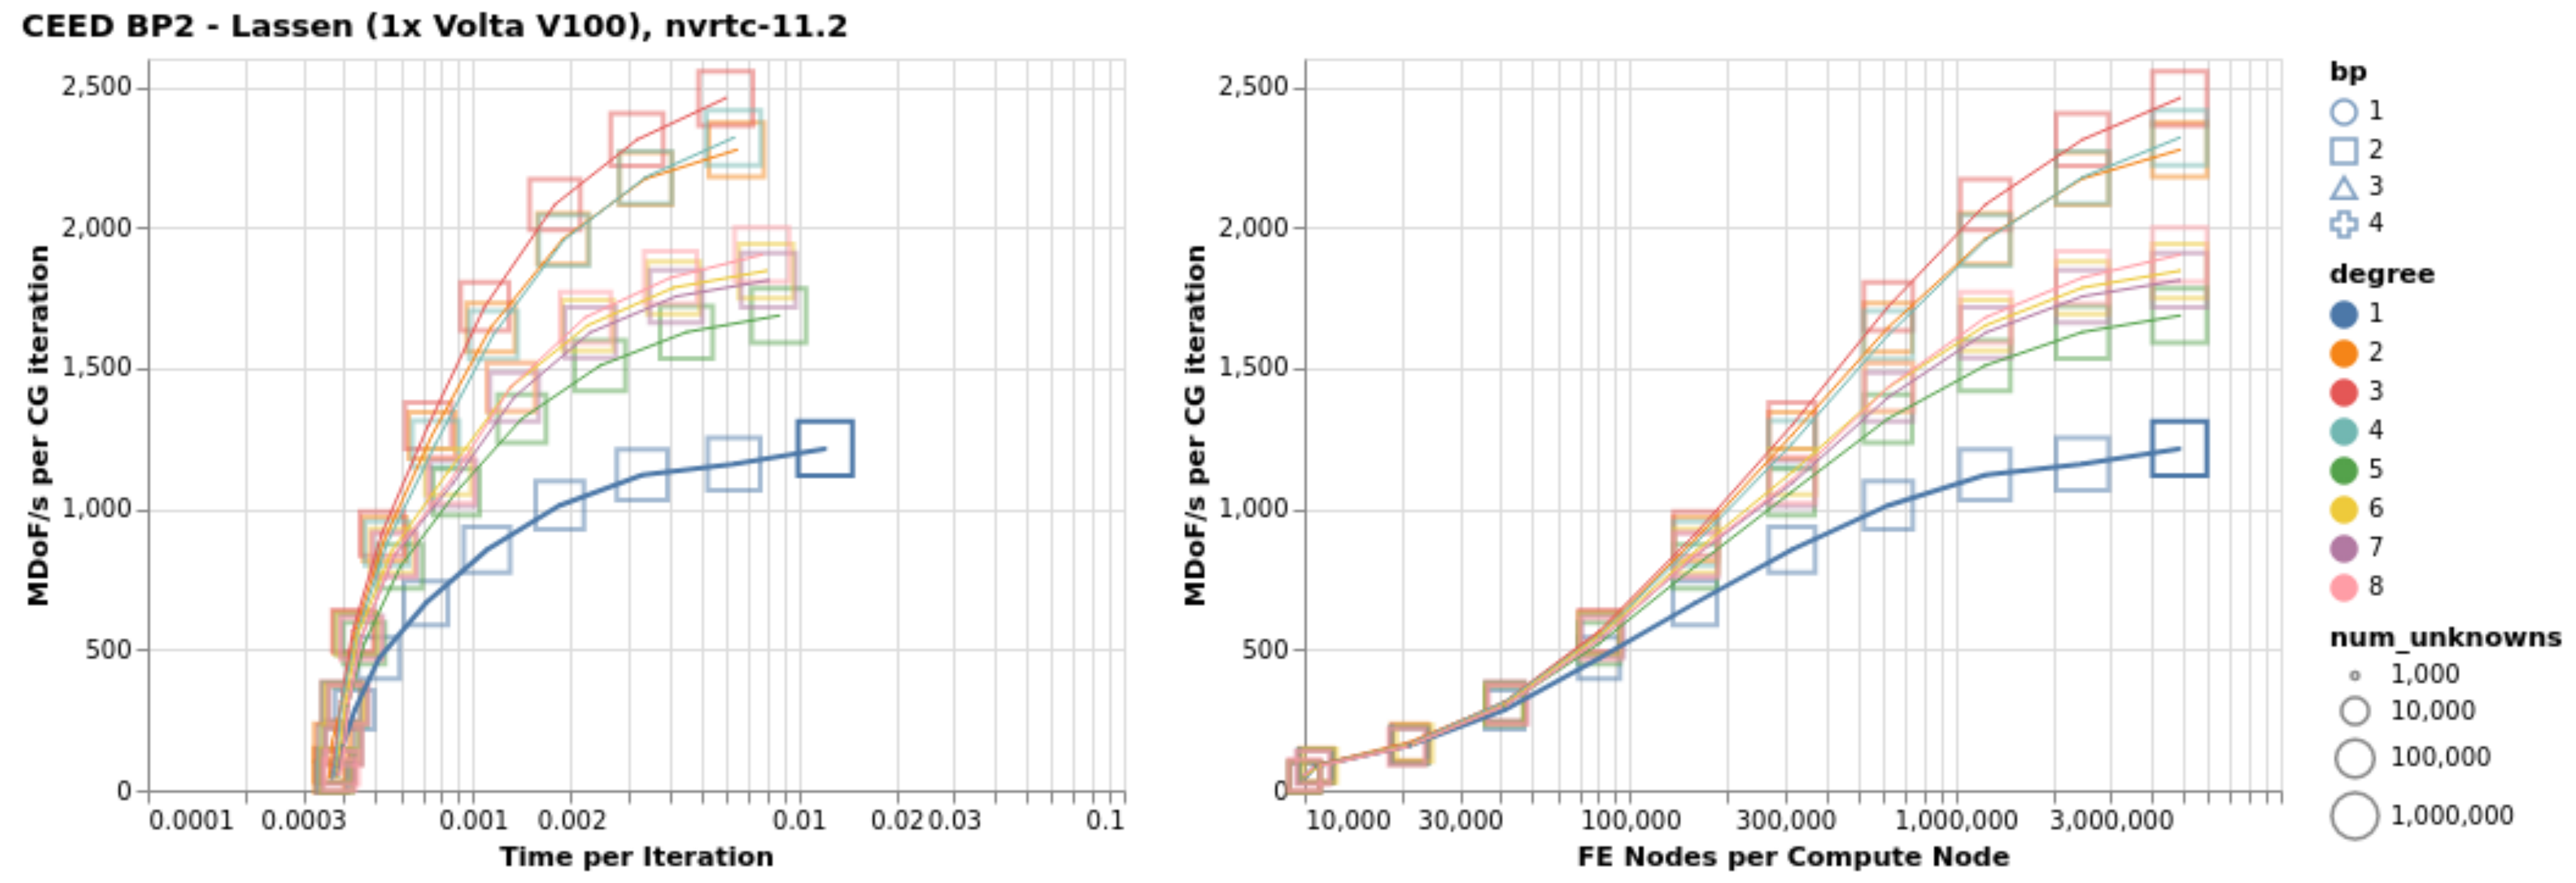
\includegraphics[width=.99\linewidth]{../img/cudaGenBP2Clip}
\caption{CEED Benchmark BP2 - NVIDIA V100}
\label{fig:gpu-bp2}
\end{figure}

\begin{figure}[ht!]
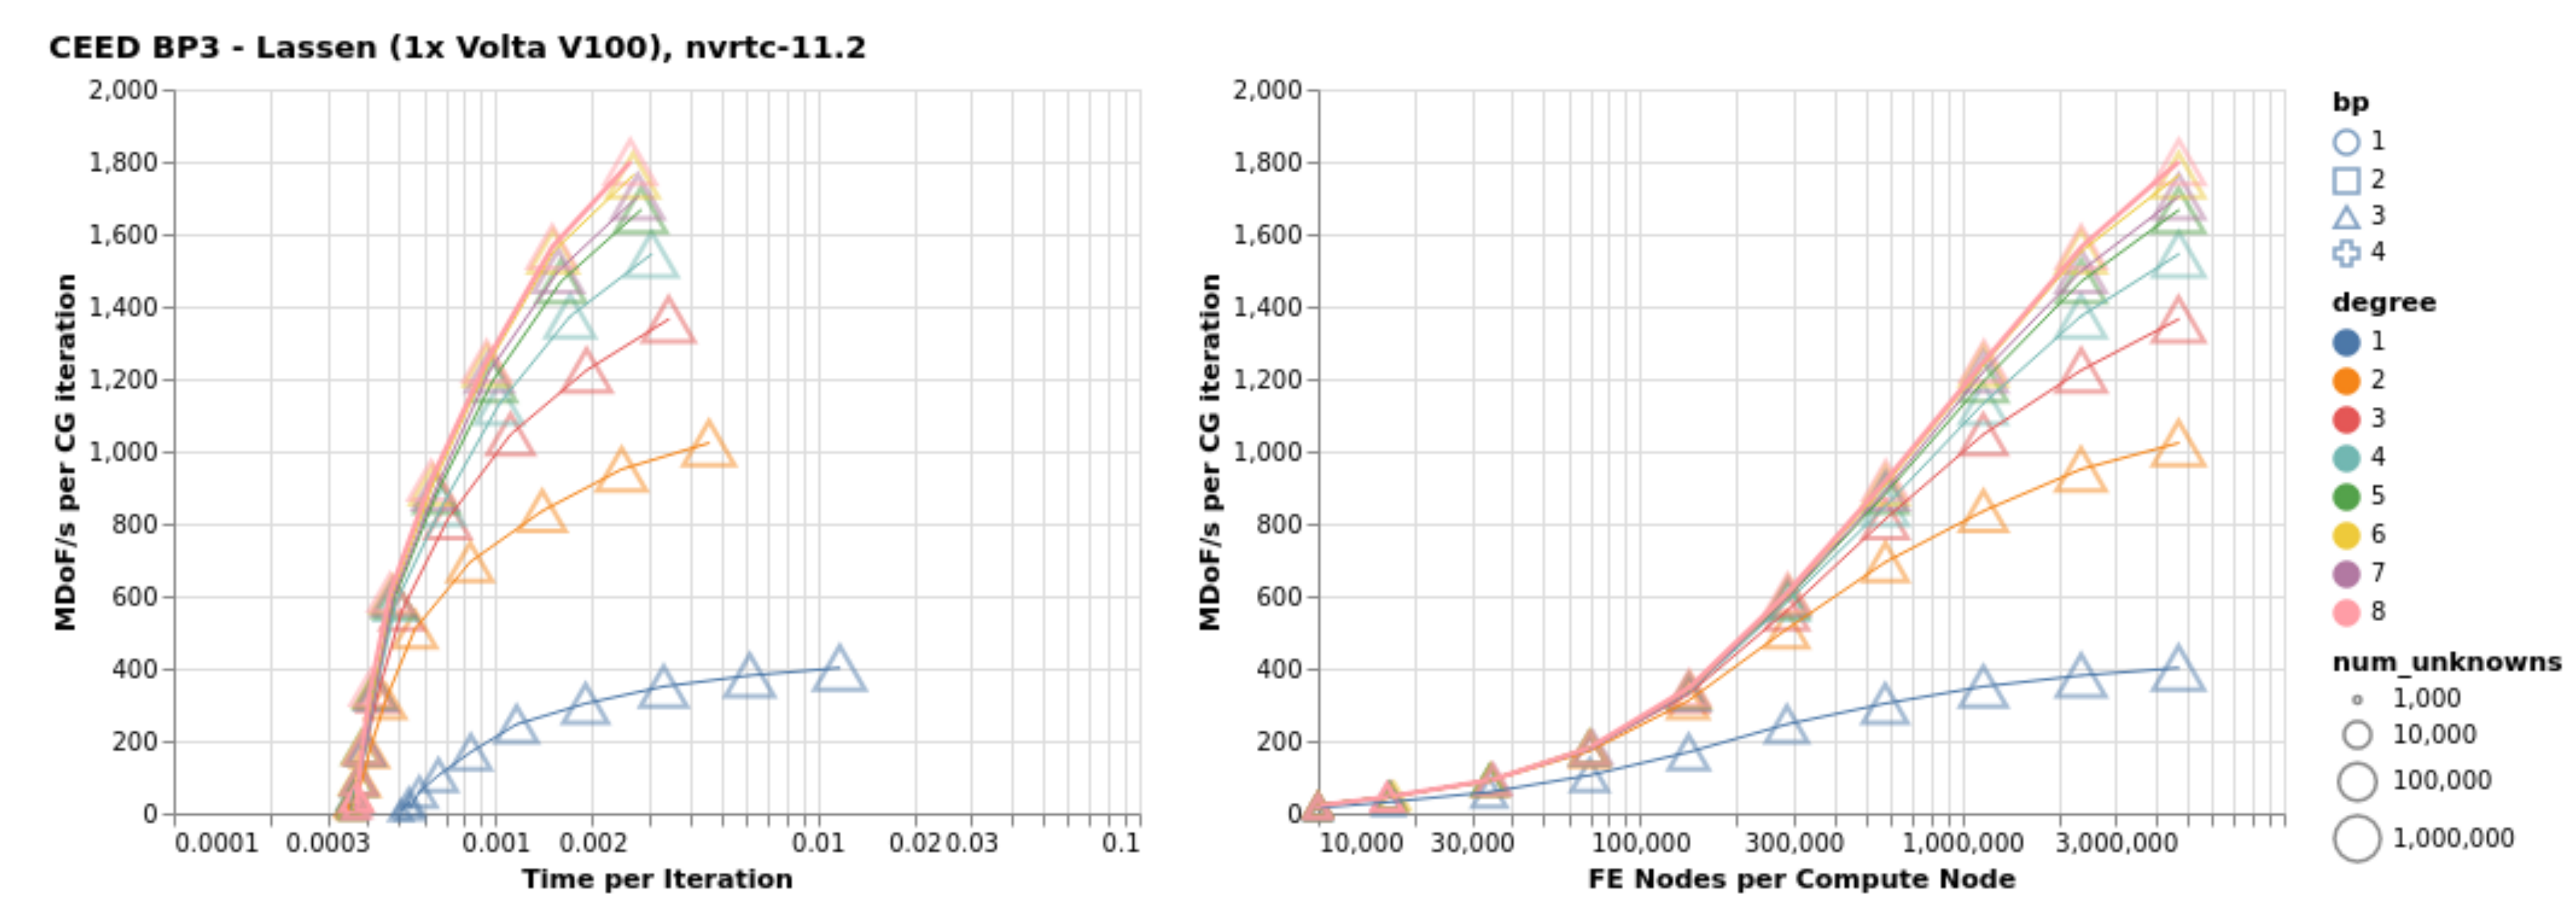
\includegraphics[width=.99\linewidth]{../img/cudaGenBP3Clip}
\caption{CEED Benchmark BP3 - NVIDIA V100}
\label{fig:gpu-bp3}
\end{figure}

\begin{figure}[ht!]
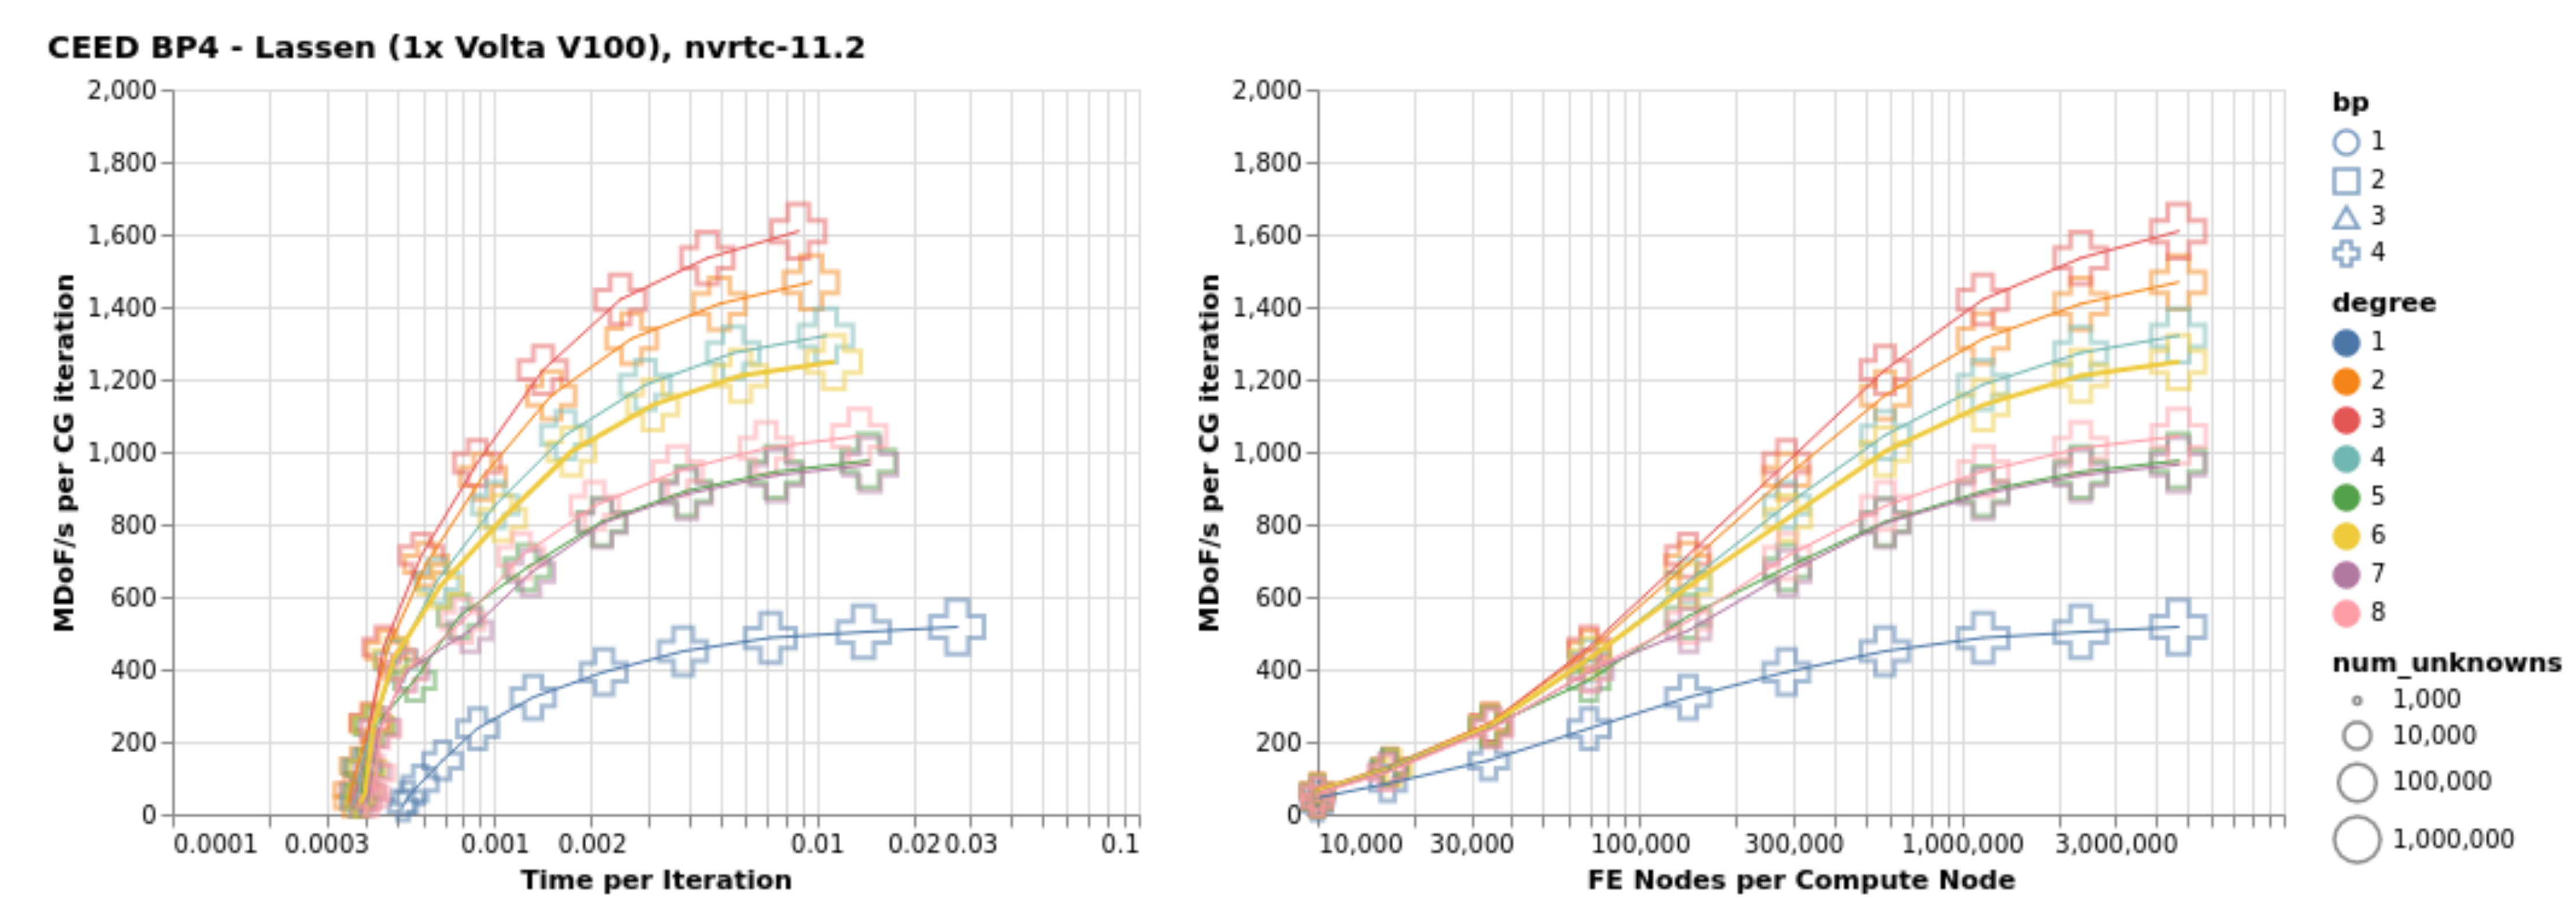
\includegraphics[width=.99\linewidth]{../img/cudaGenBP4Clip}
\caption{CEED Benchmark BP4 - NVIDIA V100}
\label{fig:gpu-bp4}
\end{figure}

~\\
The GPU performance study was conducted on a node with two-socket IBM POWER9 and four NVIDIA Volta V100s on the Lassen system at Lawrence Livermore National Laboratory.
Figures \ref{fig:gpu-bp1}, \ref{fig:gpu-bp2}, \ref{fig:gpu-bp3}, and \ref{fig:gpu-bp4} show the results of this performance study.
Each socket contains 22 CPU cores with a base clock speed of 3.45 GHz and each GPU has 5120 CUDA cores with a total of 256 GB memory fer each node.
CUDA-aware Spectrum MPI was used with PETSc \cite{petsc-user-ref} version 3.15 and libCEED \cite{libceed} version 0.9.

libCEED used the CUDA code generation backend, \lstinline{\gpu\cuda\gen}.
In the code generation backends, the user source code for the application of the weak form at the quadrature points ${\color{applegreen}\mathbf{D}}$ is JiT compiled into a single kernel that represents the action of the full operator ${\color{burgundy}\mathbf{A}}$.
This approach reduces latency from additional kernel launches and helps provide the best performance of NVIDIA and AMD GPU hardware.

As before, throughput increases as polynomial order increases.
The the high throughput with high latency indicates that the architecture weak scales effectively, while high throughput with low latency would indicate that this architecture demonstrates good strong scaling.

The specific performance tradeoffs depend upon the hardware, and these benchmark problems help inform users about the performance capabilities of their hardware for high-order matrix-free representations of PDE operators.
